\documentclass{report}
\usepackage[margin=1in, paperwidth=8.5in, paperheight=11in]{geometry}
%Math packages%
\usepackage{amsmath}
\usepackage{amsthm}
%Spacing%
\usepackage{setspace}
\onehalfspacing
%Lecture number%
\newcommand{\lectureNum}{11}
%Variables - Date and Course%
\newcommand{\curDate}{January 27, 2017}
\newcommand{\course}{MATH 239}
\newcommand{\instructor}{Luke Postle}
%Defining the example tag%
%\theoremstyle{definition}%
\newtheorem{ex}{Example}[section]
%Setting counter given the lecture number%
\setcounter{chapter}{\lectureNum{}}
%Package for drawing graphs%
\usepackage{tikz}
\usepackage{verbatim}
\usetikzlibrary{arrows}

\begin{document}
%Note title%
\begin{center}
\begin{Large}
\textsc{\course{} | Lecture \lectureNum{}}
\end{Large}
\end{center} 
\noindent \textit{Bartosz Antczak} \hfill
\textit{Instructor: \instructor{}} \hfill
\textit{\curDate{}}
\rule{\textwidth}{0.4pt}

% Actual Notes%
\subsubsection{Review of Last Lecture}
We proved a theorem:
\begin{center}
\textit{G is bipartite if and only if G has no odd cycles}
\end{center}
A polynomial-time algorithm for determining if $G$ is bipartite:
\begin{enumerate}
\item Find a spanning tree $T_i$ of each component $G_i$ of $G$
\item Pick a root $r_i$ for each $T_i$
\item Find $A_i = \{v \in V(T_i) : d(v, r_i) \,\, \mathrm{is \,\,even}\}$ and $B_i = \{v \in V(T_i) : d(v, r_i) \,\, \mathrm{is\,\, odd}\}$
\item Let $A = \cup_i A_i,\, B = \cup_i B_i$
\item If all edges have one end in $A$ and other end in $B$: return yes and the bipartition $(A, B)$ to verify this
\item Otherwise, there exists an edge $e = uv$ with both ends in same partition: now find a path $P$ from $u$ to $v$ in the tree $T_i$ containing $u$ and $v$ and return no! The odd cycle $C = P+e$ verifies that $G$ is not bipartite
\end{enumerate}
\section{Bridges}
A \textbf{bridge} of a graph $G$ is an edge $e$ such that $G - e$ has more components than $G$.
\begin{ex}
Various graphs with their respective bridges labelled `$\beta$'
\end{ex}
%Example 1%
\begin{center}
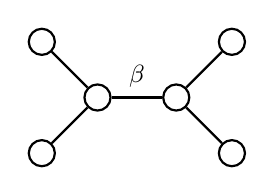
\begin{tikzpicture}[-,auto,node distance=1cm,
                    thick,main node/.style={circle,draw,font=\sffamily\small}]

  \node[main node] (1) {};
  \node[main node] (2) [below left of=1] {};
  \node[main node] (3) [above left of=1] {};
  \node[main node] (4) [right of=1] {};
  \node[main node] (5) [below right of=4] {};  
  \node[main node] (6) [above right of=4] {};    
  \path[every node/.style={font=\sffamily\small}]
    (1) edge (2)
    	edge (3)
    	edge node [above] {$\beta$} (4)
    (4) edge (5)
    	edge (6);
\end{tikzpicture}
%Example 2 (non-connected graph)%
$\qquad\qquad\qquad\qquad$ %<-- Spacing%
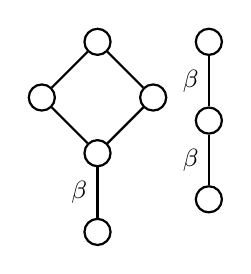
\begin{tikzpicture}[-,auto,node distance=1cm,
                    thick,main node/.style={circle,draw,font=\sffamily\small}]

  \node[main node] (1) {};
  \node[main node] (2) [below left of=1] {};
  \node[main node] (3) [below right of=1] {};
  \node[main node] (4) [below right of=2] {};
  \node[main node] (5) [below of=4] {};  
  \node[main node] (6) [above right of=3] {};
  \node[main node] (7) [below of=6] {};  
  \node[main node] (8) [below of=7] {};  
  \path[every node/.style={font=\sffamily\small}]
    (1) edge (2)
    	edge (3)
    (4) edge (2)
    	edge (3)
    	edge node [left] {$\beta$} (5)
    (7) edge node [left] {$\beta$} (6)
    	edge node [left] {$\beta$} (8);
\end{tikzpicture}
\end{center}
\subsection{Theorem}
%Theorem numbers do not coincide with the course notes%
\begin{center}
\textit{An edge $e=uv$ is not a bridge of graph G if and only if there is a cycle $C$ of $G$ that contains e}
\end{center}
(Proof is on the next page).
\newpage
\subsubsection{Proof:}
\begin{center}
edge $e = uv$ is not a bridge
$$\iff$$
$u$ and $v$ are in the same component of $G-e$
$$\iff$$
there is a path $P$ in $G-e$ from $u$ to $v$
$$\iff$$
there is a cycle $C$ of $G$ that contains $e$
\end{center}
\subsection{Corollary}
\begin{center}
\textit{Graph G is a forest if and only if all edges are bridges}
\end{center}
Also similarly: when $G$ is connected,
\begin{center}
\textit{G is a tree if and only if all of its edges are bridges}
\end{center}
\section{Weighted Graphs}
A \textbf{weighted graph} is a graph $G$ with a weight function $w$ on the edges of $G$ (for the purposed of this class, we assume $w$ is non-negative).
\begin{ex}
A graph with a weight on each edge
\end{ex}
%Example 2%
\begin{center}
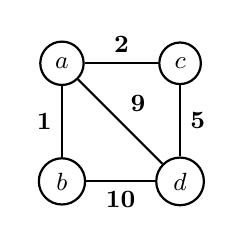
\begin{tikzpicture}[-,auto,node distance=1.5cm,
                    thick,main node/.style={circle,draw,font=\sffamily\small}]

  \node[main node] (1) {$a$};
  \node[main node] (2) [below of=1] {$b$};
  \node[main node] (3) [right of=1] {$c$};
  \node[main node] (4) [right of=2] {$d$}; 
  \path[every node/.style={font=\small}]
    (1) edge node [left]{\textbf{1}} (2)
    	edge node [above]{\textbf{2}} (3)
    (4) edge node [below] {\textbf{10}} (2)
    	edge node [right] {\textbf{5}} (3)
    	edge node [above right] {\textbf{9}} (1);
\end{tikzpicture}
\end{center}
\noindent Weighted graphs model
\begin{itemize}
\item Time taken to travel between nodes
\item Distance between nodes
\item Cost required to travel between nodes
\end{itemize}
\subsubsection{Question 1}
Finding the shortest paths in weighted graphs is useful, and there are very efficient algorithms that do this. Let's consider the weight of each edge in terms of cost. Can we find a cheapest cost set of edges connecting all vertices efficiently? (We can interpret this question as the edges being roads and vertices being cities, for a practical example)
\subsubsection{Observation 1}
Let's consider the graph from example 11.2.1, observe that the cheapest set of edges would include 1, 2, and 5. From this observation, we can conclude that a cheapest cost set has no cycles, because a cycle will always contain at least one extra edge not needed to connect all vertices.\\Since this edge set must connect all vertices and contain no cycle, the cheapest cost set is actually a \textit{spanning tree}. From this, we derive a definition:
\subsection{Minimum Weight Spanning Tree (MST)}
A tree $T$ is an \textbf{MST} of a weighted graph $G$ if it has a minimum weight $\displaystyle\left(\sum_{e \in E(T)} w(e)\right)$ among all spanning trees. \\
How can we find an MST? We can use \textit{Prim's Algorithm}.
\subsubsection{Prim's Algorithm}
\begin{itemize}
\item Pick a vertex $v$ and put it in our spanning tree $T$ (initially will only contain $v$)
\item While $T$ is not a spanning tree:
\begin{itemize}
\item Pick an edge $e$ in $\delta(V(T))$ of \textit{least weight}
\item Set $T := T + e$
\end{itemize}
\end{itemize}
\begin{ex}
Applying Prim's Algorithm on the weighted graph from example 11.2.1
\end{ex}
\begin{itemize}
\item Let's pick vertex $c$ to be our tree $T$. The weight of each edge in $\delta(T)$, $\{ca, cd\}$, is respectively $\{2, 5\}$. We choose the lighter edge $ac$ to be added to $T$
\item Now $\delta(T) = \{ab, ad, cd\}$. We choose $ab$, which is the lightest
\item Finally, $\delta(T) = \{ad, cd\}$, and we choose $cd$. Now all vertices are connected, and we have constructed an MST
\end{itemize}
\subsection{Theorem}
\begin{center}
\textit{The graph constructed using Prim's algorithm is always an MST}
\end{center}
\subsubsection{Proof:}
Let $T_0$ be the graph constructed using Prim's algorithm, and let $e_1, e_2, \cdots, e_{n-1}$ be all of the edges of $T_0$ in the order they are added to $T$. Let $T$ be an MST of graph $G$ such that if edge $k$ is the smallest $i$ such that $e_i \not\in E(T)$ that $k$ is maximized among all MST's. \\
\textbf{Claim:} $T_0 = T$ and hence $k$ does not exist.
\begin{itemize}
\item \underline{Proof of Claim}: suppose that $k$ \textit{does} exist. That is, $e_1, e_2, \cdots, e_{k-1} \in E(T)$ but $e_k \not\in E(T)$. I claim that there exists a spanning tree $T^\prime$ that uses $e_k$ instead of another edge $f$ in $\delta(V(T))$ and otherwise equals to $T$. But now $w(T^\prime) \leq w(T)$ since $e_k$ had the smallest weight in $\delta(V(T))$. But now $T^\prime$ uses $e_1, \cdots, e_k$ and so $T$ is not maximal, which is a contradiction. Ergo, $k$ does not exist. Thus, $T_0 = T$, which proves our statement.
\end{itemize}

%END%
\end{document}